\documentclass{bmstu-pr}

\begin{document}

\prtitle{Классификация методов подсчета\\информационной энтропии}{Хамзина
Регина Ренатовна}{ИУ7-73Б}{Оленев Антон Александрович}

\begin{frame}
    \frametitle{Цель и задачи}

    \textbf{Цель:} классификация методов подсчета информационной энтропии.

    \textbf{Задачи:}
    \begin{itemize}
		\item провести анализ предметной области: рассмотреть основные определения, изучить свойства информационной энтропии и ее связь со сжатием данных;
		\item описать существующие методы подсчета информационной энтропии;
		\item выделить критерии сравнения описанных методов;
		\item провести сравнение методов по выделенным критериям.
    \end{itemize}
\end{frame}

\begin{frame}
    \frametitle{Передача информации}
    
	\begin{figure}[h]
    		\centering
    		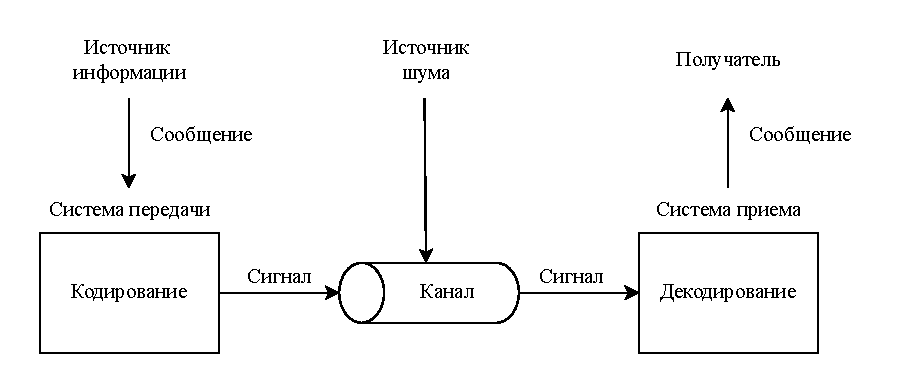
\includegraphics[width=0.6\textwidth]{img/transmission.pdf}
	\end{figure}
	
	\begin{equation}
		H(X) = -\sum_{i = 1}^n (p_{i} \cdot \log_{a}p_{i}),
	\end{equation}
	
	где $n \in \mathbb{N}$, $p_{i} = P(X \sim x_{i})$, $\sum_{i = 1}^n p_{i} = 1$, $a > 1$.

\end{frame}

\begin{frame}
    \frametitle{Связь энтропии и сжатия данных}
    
	\begin{figure}[h]
    		\centering
    		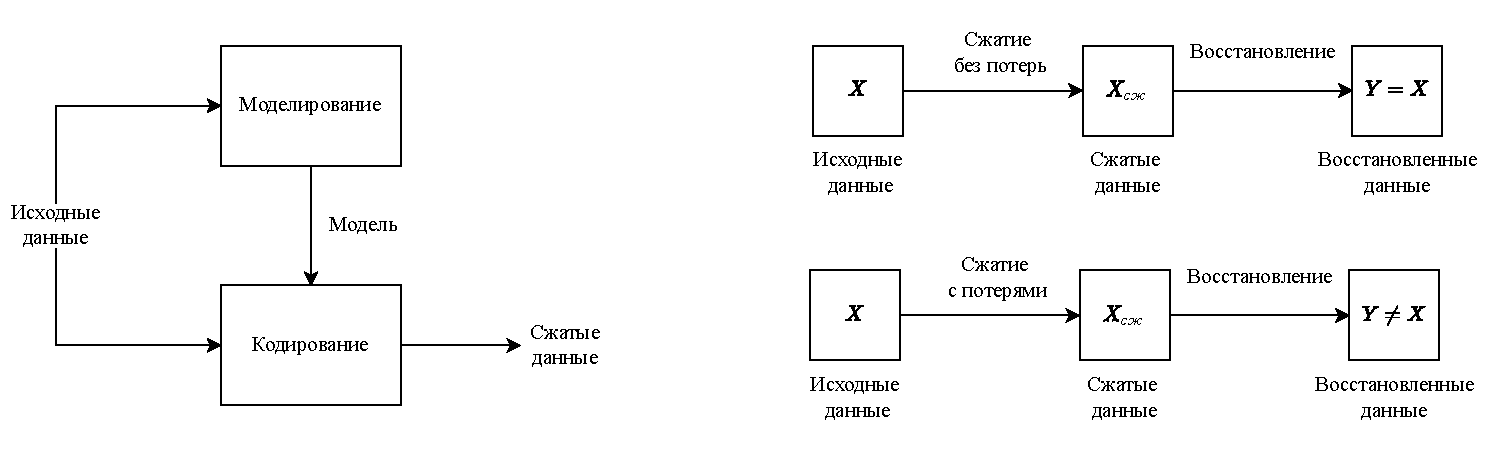
\includegraphics[width=0.9\textwidth]{img/compression.pdf}
	\end{figure}

	\begin{equation}
		K_{\text{сж}} = \frac{L_{\text{исх}}}{L_{\text{сж}}},
	\end{equation}

	где $L_{\text{исх}}$ --- объем исходных данных $X$, $L_{\text{сж}}$ --- объем сжатых данных~$X_{\text{сж}}$.
\end{frame}

\begin{frame}
    \frametitle{Метод скользящего окна}
    
	\begin{figure}[h]
    		\centering
    		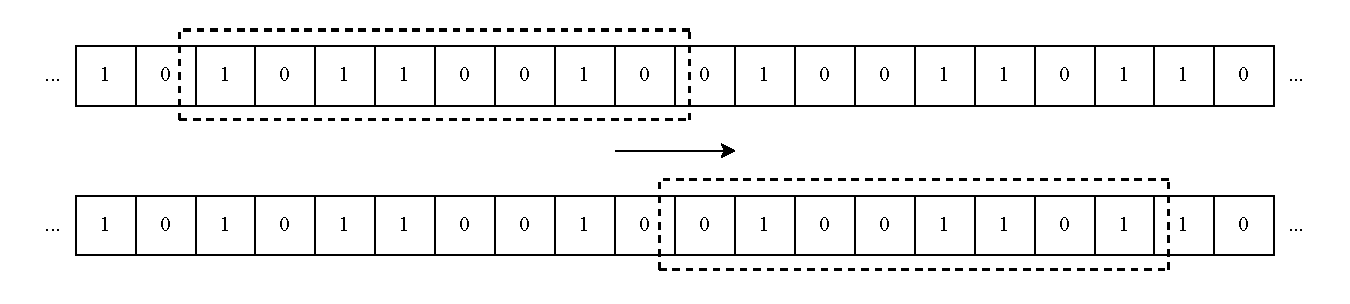
\includegraphics[width=0.8\textwidth]{img/sliding-window.pdf}
	\end{figure}

 	\begin{equation}
		H(X) = -\sum_{i = 0}^{255} (p_{i} \cdot \log_{2}p_{i}),
	\end{equation}
	
	где $p_{i} = \frac{k_{i}}{N}$ --- вероятность появления байта в массиве байтов размером $N$, $k_{i}$ --- число вхождений байта в массив байтов.
\end{frame}

\begin{frame}
    \frametitle{Биномиальный метод}
    
	\begin{figure}[h]
    		\centering
    		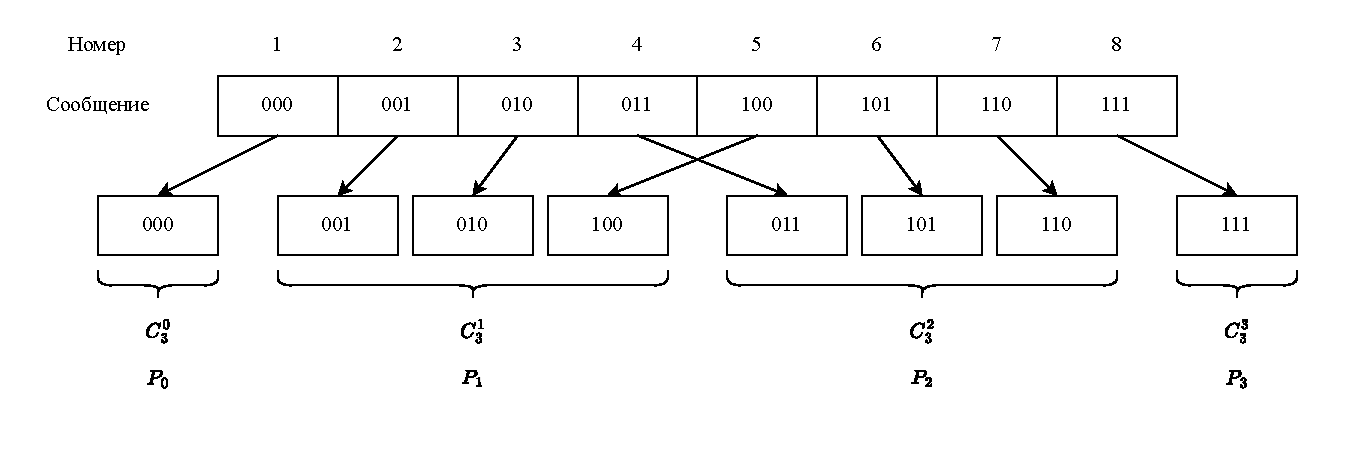
\includegraphics[width=0.7\textwidth]{img/binomial-method.pdf}
	\end{figure}
    
	\begin{equation}
		H(X) = -\sum_{k = 0}^n (C_{n}^k \cdot P_{k} \cdot \log_{2}P_{k}),
	\end{equation}
	
	где $P_{k} = p^k \cdot (1 - p)^{(n - k)}$, $C_{n}^k = \frac{n!}{k! \cdot (n - k)!}$.

\end{frame}

\begin{frame}
    \frametitle{Сравнение методов}
    
	\begin{table}[h]
    			\begin{center}
        		\begin{tabular}{|l|l|l|l|l|}
        			\hline
            		\multicolumn{1}{|c}{\textbf{Метод}} & 
            		\multicolumn{1}{|c|}{\textbf{K1}} &
            		\multicolumn{1}{c|}{\textbf{K2}} &
            		\multicolumn{1}{c|}{\textbf{K3}} & 
            		\multicolumn{1}{c|}{\textbf{K4}} \\ \hline
            		Скользящего окна &  $O(N + 2^n)$ & - & + & $2^n$ \\ \hline
            		Биномиальный &  $O(N + n)$ & + & + & $2 \cdot (n + 1)$ \\ \hline
        		\end{tabular}
    		\end{center}
	\end{table}
	
	\begin{itemize}
		\item K1 --- временная сложность;
		\item K2 --- необходимость вычисления факториала;
		\item K3 --- возможность распараллеливания вычислений;
		\item K4 --- объем требуемой дополнительной памяти.
	\end{itemize}

\end{frame}

\begin{frame}
    \frametitle{Заключение}
    Цель научно-исследовательской работы достигнута.
    
	При написании данной работы:

	\begin{itemize}
		\item проведен анализ предметной области: рассмотрены основные определения, изучены свойства информационной энтропии и ее связь со сжатием данных;
		\item описаны существующие методы подсчета информационной энтропии;
		\item выделены критерии сравнения описанных методов;
		\item проведено сравнение методов по выделенным критериям.
	\end{itemize}
\end{frame}

\end{document}